\chapter[Unveiling DNA Translocation in Pristine Graphene Nanopores: Understanding Pore Clogging via Polarizable Simulations]{Unveiling DNA Translocation in Pristine Graphene Nanopores: Understanding Pore Clogging via Polarizable Simulations \protect\footnote[5]{This chapter has been published as \textbf{H., Hemanth} and Mallajosyula*, S.S.; Unveiling DNA Translocation in Pristine Graphene Nanopores: Understanding Pore Clogging via Polarizable Simulations; {\textit{ACS Appl. Mater. Interfaces}, 2023, \textbf{47}, 55095–55108}}}

\section[Introduction]{Introduction}
Whole genome sequencing (WGS) is recognized as a key step in the advancement of modern medicine, with major implications in the development of personalized treatment protocols.\supercite{dewey_clinical_2014} WGS would enable the early identification of genetic disorders and would help in providing suitable medical attention to the general public.\supercite{abubaker_bagabir_covid-19_2022} In the recent years, the importance of WGS was highlighted in tracking the spread of novel coronavirus (Covid-19) and the subsequent development of suitable vaccines to curb the spread of the infection.\supercite{chen_next-generation_2021} WGS enabled the identification of the variants of concern of the severe acute respiratory syndrome coronavirus 2 (SARS-CoV-2) as the virus mutated, which greatly influenced the policy response towards the pandemic situation.\supercite{abubaker_bagabir_covid-19_2022,chen_next-generation_2021} Key to WGS is the requirement of a rapid, accurate and cost-effective sequencing platform.\supercite{giani_long_2020} Traditional efforts on sequencing the DNA are based on the Sanger method, where the DNA strand of interest is fragmented, and amplified before being sequenced.\supercite{sanger_dna_1977} The sequence of the original DNA strand is then recovered based on the overlaps in the fragmented DNA. The traditional sanger-based methods are time-consuming and laborious which lead to the development of next generation sequencing (NGS) technologies that use massively parallel sequencing approaches.\supercite{manyana_hiv-1_2021} However even the NGS methods rely on the fragmentation of the original DNA strand.

Nanopores offer an alternative platform for DNA sequencing that does not involve strand fragmentation. The basic principle of nanopore sequencing is that the analytes enter the nanopore under an applied potential which alters the flow of ions through the nanopore resulting in blockades of the ionic current.  These resultant ionic current blockades are analysed to identify the analyte. Two variants of nanopores have been explored for DNA sequencing (i) Biological nanopores and (ii) Solid state nanopores. Biological nanopores are formed by the self-assembly of protein, peptides or even DNA scaffolds in lipid bilayers or polymer membranes and have been successfully used in sequencing technology.\supercite{hu_biological_2021} However, one of the key limitations of biological nanopores is that they are very susceptible to changes in pH and temperature and cannot be readily reused, which affects their scope of application.\supercite{haque_solid-state_2013} Solid state nanopores, on the other hand provide a stable alternative to the biological nanopores. Solid state nanopores are typically fabricated using techniques like electron milling,\supercite{storm_fabrication_2003} laser-based etching\supercite{gilboa_optically-monitored_2018} and dielectric breakdown of solid membranes,\supercite{waugh_solid-state_2020} which allows one to control the dimensions of the nanopore. Initial studies using conventional silicon based nanopores were not successful in DNA sequencing due to the relatively large thickness of the nanopore membrane that corresponded to multiple nucleobases occupying the nanopore at the same time leading to a loss of resolution.\supercite{li_dna_2003} This led to the search for substrates with thickness that would allow single nucleobases to occupy the nanopore while translocating through it. 

The discovery of graphene\supercite{geim_graphene_2009} and related 2D materials\supercite{novoselov_two-dimensional_2005} of sub nanometre thickness ignited the possibility of using such materials as suitable membranes for DNA sequencing. These 2D membranes in principle address the challenges of stability associated with biological nanopores\supercite{mayer_biological_2022} and membrane thickness associated with silicon based solid state nanopores.\supercite{li_dna_2003} In 2010 a series of initial experiments demonstrated the detection of DNA passing through graphene nanopores.\supercite{schneider_dna_2010,merchant_dna_2010,garaj_graphene_2010} These experiments led to numerous other studies exploring 2D materials for DNA sequencing technologies. We refer the readers to excellent review articles which summarize the progress made in DNA sequencing using graphene and other 2D materials.\supercite{xue_solid-state_2020,qiu_nanopores_2021} Despite the initial excitement the key aim of achieving single-base resolution using graphene nanopores has remained elusive. One of the major issues has been the translocation dynamics of DNA in the nanopore.\supercite{venkatesan_nanopore_2011} Translocation speeds of 20,000-100,000 basepairs/ms have been observed in typical graphene based nanopore experiments. These speeds are generally observed due to the very large pore diameters (3-25 nm)\supercite{schneider_dna_2010,merchant_dna_2010,garaj_graphene_2010} and contaminated graphene lattices used in these studies. On the other hand, Dekker and co-workers reported that clean crystalline graphene nanopores are prone to severe clogging and pore closures for pore diameters ranging from 3 nm to 20 nm.\supercite{schneider_tailoring_2013} These crystalline graphene pore diameters are ideal for observing translocation speeds of 1-100 basepairs/ms which are ideal for achieving single base detection. Understanding the atomistic interactions responsible for the pore clogging and translation dynamics would provide insight into the future development of graphene based nanopores.

Molecular dynamics (MD) simulations studying the translocation dynamics of both single-stranded DNA (ssDNA) and double-stranded DNA (dsDNA) in graphene nanopores have provided atomistic level insights into the translocation events.\supercite{barati_farimani_dna_2017} In a seminal work Aksimentiev and co-workers used MD simulations to address the suitability of graphene nanopores for sequencing ssDNA.\supercite{wells_assessing_2012} In their simulations and in most MD simulations subsequently the graphene nanopore is represented as a clean crystallographic nanopore with the graphene lattice being preserved up to the edges of the nanopore. Aksimentiev and co-workers observed that ssDNA was found to adhere to the graphene surface resulting in 2D diffusion of the adhered DNA on the graphene surface, limited translocation events and even clogging of the pore that required transmembrane bias of about 500 mV to unclog and complete the translocation event. In some cases, the bias voltage had to be increased to 800 mV to complete the translocation event. The pore diameter for which translocation events were observed was 16 Å. Many of these observations were later corroborated in the experimental study by Dekker and co-workers.\supercite{schneider_tailoring_2013,heerema_graphene_2016} However one significant difference between the two studies was the severity of the pore clogging in the experimental study which was not captured in the MD simulations. Using a pore diameter of 50 Å, which was significantly larger than the 16 Å diameter used in the MD studies, Dekker and co-workers observed significant pore clogging which could not be relieved even under the application of multiple large 1V pulses.\supercite{schneider_tailoring_2013} In the MD simulations ramping up the bias by 300 mV was sufficient to progress the translocation event. Subsequent MD studies have also reported a smooth translocation of DNA strands via the nanopores under the application of a bias voltage.\supercite{tyagi_revealing_2019} We note that all these simulations were performed using the additive (non-polarizable) force-fields (FF), which do not account for charge transfer and polarization effects due to the fixed-point charges associated with the atoms in the additive (non-polarizable) FF. This becomes especially crucial when trying to describe the large $\pi$-cloud above the graphene surface. A way to address this issue is the inclusion of polarization into MD simulations. 

The importance of polarizable description of surfaces, especially treating the induced charges in the presence of solvent and counter ions has been recognized when describing interfacial phenomenon\supercite{kondrat_theory_2023,siepmann_influence_1995}. The Drude model presents a simple extension of the potential which can be easily implemented and remains compatible with common bio-molecular force fields, as described by the implementation of the Drude model potential for metallic surfaces.\supercite{geada_insight_2018} Drude parameters have also been developed to describe graphene surfaces.\supercite{ho_polarizability_2013,misra_insights_2017} Striolo et. al. targeted the per atom polarizability of 0.867 Å\textsuperscript{3} for graphene C atoms based on ab-initio calculations of the out-of-plane polarization of multi-layer graphene in vacuum and did not include solvation effects.\supercite{ho_polarizability_2013} In an unrelated study Blanksctein et. al. used a site polarizability of 1.139 and a thole scaling factor of 1.507 to describe the graphene C atoms to capture the wetting of the graphene surfaces by water and reproduce experimentally observed contact angles.\supercite{misra_insights_2017} These Drude parameters were not tested to study $\pi$-$\pi$ interactions between graphene surfaces and aromatics. Towards this endeavour we reported the development of Drude parameters for describing a polarizable graphene sheet which remains compatible with the existing parameters in the CHARMM Drude polarizable force field that encompasses proteins, nucleic acids, carbohydrates and small molecules.\supercite{h_polarization_2021} We used a site polarizability of 1.615 and a thole scaling factor of 1.195 to describe the C atoms in the graphene sheet. These parameters are consistent with the description of aromatics in the CHARMM Drude polarizable force field.\supercite{lopes_polarizable_2007} The parameters were tested to reproduced water-binding energies and nucleobase-graphene $\pi$-$\pi$ interaction energies. The developed parameters were first used to study the aggregation behavior of nucleobases dispersed on a graphene support.\supercite{h_polarization_2021} The polarizable simulations were able to capture experimentally observed $\pi$-$\pi$ stacking interactions amongst Guanine nucleobases\supercite{varghese_binding_2009} and the formation of ordered self-assemblies for Adenine and Cytosine nucleobases.\supercite{otero_elementary_2008,wandlowski_structure_1996} The parameters were also used to study the concentration dependent self-assembly of cytosine nucleobases on 2D graphene support.\supercite{h_capturing_2022} Wherein, in the low surface loading concentration (0.25 M) limit the simulations were able to capture ordered self-assemblies that were consistent with the experimental assemblies of cytosine nucleobases adsorbed on 1-octanol/HOPG solid-liquid interfaces\supercite{xu_coadsorption_2006} and Au(111) surfaces\supercite{otero_elementary_2008,wandlowski_structure_1996} observed via HR-STM-imaging. Additionally, the developed parameters were also used to capture the solvation dynamics of ions at the graphene electrolyte interface.\supercite{h_capturing_2023} The polarizable simulations were able to capture both the size and charge dependent ion-graphene interactions. In particular, the Drude parameters were able to reliably capture the anion-graphene interactions. We note that all these effects which were captured by polarizable simulations are severely underestimated in the additive (non-polarizable) simulations.\supercite{h_polarization_2021,h_capturing_2022,h_capturing_2023} Polarizable force fields have also been found to accurately describe the thermodynamics of ion permeation in biological nanopores which could not be described by additive (non-polarizable) simulations.\supercite{prajapati_computational_2020} In this study, we use polarizable simulations for the first time to study the translocation dynamics of ssDNA through a graphene nanopore. 

\section{Computational Methodology}
We constructed four single stranded DNAs (ssDNA), as twenty nucleoside homopolymers of deoxy-adenosine (dA\textsubscript{20}), deoxy-guanosine (dG\textsubscript{20}), deoxy-cytidine (d\textsubscript{20}) and deoxy-thymidine (dT\textsubscript{20}) using the topology information present in the Chemistry at HARvard Molecular Mechanics (CHARMM) nucleic acid force field.\supercite{hart_optimization_2012,foloppe_all-atom_2000,mackerell_all-atom_2000} A multilayer graphene, consisting of three graphene sheets in ‘A-B-A’ arrangement was constructed using Inorganic Builder plugin available in VMD.\supercite{humphrey_vmd_1996} A nanopore of radius 8 Å was constructed in the nanopore by removing the atoms within 8 angstroms of the center-of-mass (COM) of each graphene layer. Dangling bonds (bonds with unsatisfied valences) were manually identified and removed during the construction of the nanopore. Aksimentiev and co-workers investigated a series of pore geometries and observed that the step wise translocation was observed for a pore diameter of 16 Å in a 3-layer graphene system.\supercite{wells_assessing_2012} Thus, the pore radius of 8 Å was considered to remain consistent with the study by Aksimentiev and co-workers and to facilitate a direct comparison with the previous study.\supercite{wells_assessing_2012} We chose to leave the pore edges unsaturated to remain consistent with the previous study.\supercite{wells_assessing_2012} The ssDNA strand was oriented along the z-axis, with three nucleotides at the 5’-end of the strand threaded through the nanopore, to minimize the onset of translocations. The combined ssDNA-multilayer graphene system was solvated and neutralized with 1M KCl using solvate and Autoionize plugins in VMD. Representative structure depicting the system setup is presented in Figure 6.1. CHARMM36 all-atom FF was used to describe bonded and non-bonded interactions in ssDNA,\supercite{hart_optimization_2012,foloppe_all-atom_2000,mackerell_all-atom_2000} ions\supercite{beglov_finite_1994} and the multilayer graphene.\supercite{vanommeslaeghe_charmm_2009} TIP3P three-point water model\supercite{jorgensen_comparison_1983} was employed to describe water molecules in additive (non-polarizable) FF simulations. 
\begin{figure}
    \centering
    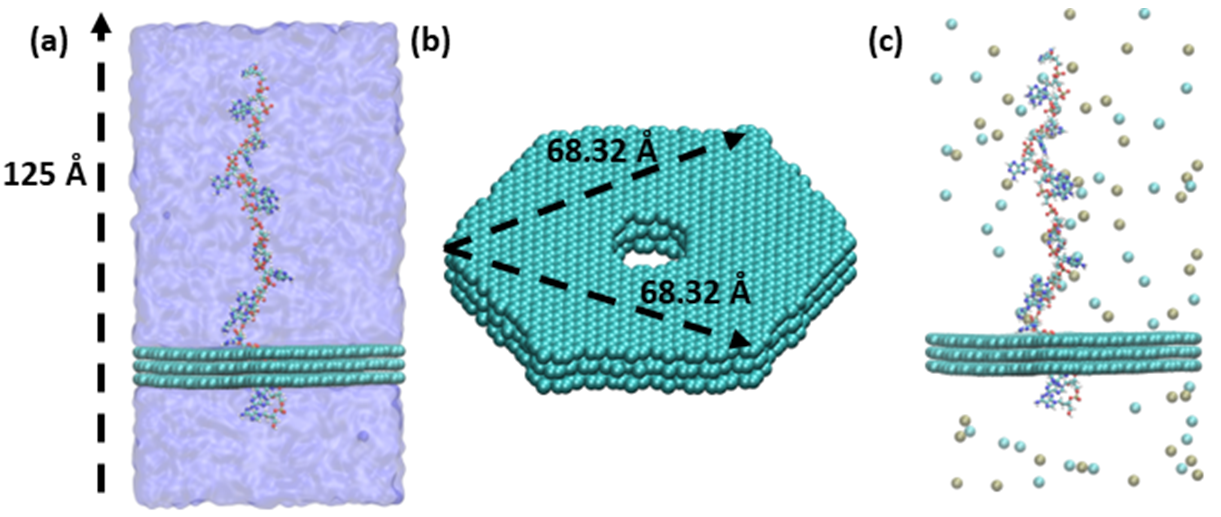
\includegraphics[width=\textwidth]{Chapter4/Figures/Figure1.png}
    \caption[Representative structures depicting the system setup for ssDNA – multilayer graphene.]{Representative structures depicting the system setup for ssDNA – multilayer graphene. (a) Side View and (b) Oblique view of the multilayer graphene to indicate periodic boundary conditions employed. (c) Complete ssDNA – multilayer graphene (water molecules are removed for clarity). All figures are prepared using VMD.\supercite{humphrey_vmd_1996}}
\end{figure}

For the polarizable simulations we employed in-house scripts to add Drude particles to the additive (non-polarizable) FF systems and generate corresponding Drude polarizable systems. Drude polarizable FF was used to describe the bonded and non-bonded interactions in ssDNA\supercite{baker_development_2011,savelyev_all-atom_2014} and ions.\supercite{lin_polarizable_2018} Parameters previously reported by us were used to describe bonded and non-bonded interactions in the multilayer graphene.\supercite{h_polarization_2021} SWM4-NDP four-point polarizable water model was used to describe the water molecules.\supercite{lamoureux_polarizable_2006} We restrained the bond lengths and bond angles in water molecules using the SETTLE\supercite{miyamoto_settle_1992} algorithm in Drude polarizable FF simulations.

All-atom MD simulations were performed using the Nanoscale Molecular Dynamics (NAMD) package.\supercite{phillips_scalable_2005} We employed a real-space cut-off of 9 Å while evaluating electrostatic interactions using Particle Mesh Ewald\supercite{darden_particle_1993} (PME) summation. Equations of motion were integrated using a time step of 1 fs for additive (non-polarizable) FF simulations and a reduced time step of 0.5 fs for Drude polarizable FF simulations. We employed a Langevin thermostat to maintain the simulated system at 298 K. An additional dual thermostat was employed to couple the Drude particles to an ice-bath at 1K. Systems were minimized for 40,000 conjugate-gradient steps to remove unfavorable contacts. The minimized geometries were further equilibrated for 2 ns in an isothermal-isobaric (NPT) ensemble followed by 3 ns in an isothermal-isochoric (NVT) ensemble.  Production runs in an isobaric-isochoric (NVT) ensemble were performed for 500 ns or till a complete translocation of the ssDNA in the additive (non-polarizable) simulations, for Drude the simulations were run for 200 ns or till a complete translocation of the ssDNA is observed. 

For the additive (non-polarizable) FF simulations, the initial applied external bias was set to 0.50 V (500 mV) for the first 100 ns of the production runs. The external bias was then increased to 0.75 V (750 mV) for the next 150 ns in the production runs. Subsequently the external biases were increased to 1.00 V, in an attempt to drive the translocation to completion. 

For the Drude polarizable FF two initial independent runs were initiated with bias voltages of 0.5 V and 1.0 V for 50 ns and 100 ns respectively. No translocations were observed during the 0.5 V runs and for the 1.0 V runs translocations were observed only for dT\textsubscript{20}. Based on these observations for effecting translocations, the initial applied external bias was set to 1.0 V for the first 20 ns of the production runs. The bias was ramped up to 1.50 V for the next 80 ns. After the completion of 100 ns the applied external bias was increased to 1.75 V in an attempt to drive the complete translocation. 

To understand the energetics of the DNA graphene interactions we also computed binding free energies corresponding to the nucleoside-graphene and the modified-nucleotide-graphene interactions using adaptive biasing force (ABF) simulations. We use a modified nucleotide (nucleotide') with phosphate at the 3’ and 5’-ends passivated by methyl groups. This was to mimic the sugar phosphate backbone and the charges observed in the single strand DNA. ABF simulations were also used to compute binding free energies of deoxy-ribose graphene interactions and dimethyl phosphate graphene interactions. For the ABF simulations, the systems were setup as a four-layered graphene block in a ‘ABAB’ stacking arrangement. The methodology for computing the binding free energies from ABF simulations were adopted from the previous work by Comer et. al, where four-layered graphene sheets were employed as a template for multi-layer graphene.\supercite{comer_predicting_2015} The initial coordinates of the nucleosides, nucleotides, deoxy-ribose sugar and dimethyl phosphate were constructed using the topology information available in the CHARMM additive (non-polarizable) FF.\supercite{hart_optimization_2012,foloppe_all-atom_2000,mackerell_all-atom_2000} In-house scripts were used to add the Drude particles to prepare the files for Drude polarizable simulations. We present a representative structure depicting the system setup in Figure 6.2. 
\begin{figure}
    \centering
    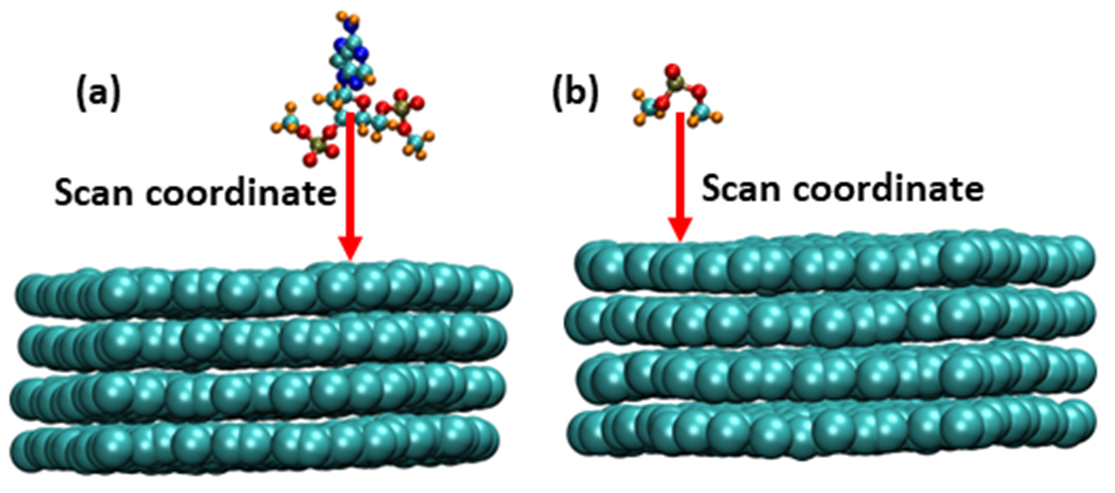
\includegraphics[width=\textwidth]{Chapter4/Figures/Figure2.png}
    \caption[Representative structures depicting the scan coordinate employed in adaptive biasing force (ABF) simulations of adenosine and dimethyl phosphate molecules]{Representative structures depicting the scan coordinate employed in adaptive biasing force (ABF) simulations of (a) adenosine molecule and (b) dimethyl phosphate molecule}
\end{figure}

To establish the inherent secondary structural preferences of ssDNA we simulated freestanding ssDNA also. Freestanding ssDNA structures were solvated in an orthorhombic box of dimensions 80 x 80 x 120 Å\textsuperscript{3}. KCl ions were added to the system using the AutoIonize plugin in VMD to bring the system to 1M concentration. The structures were minimized for 40,000 conjugate-gradient steps. The minimized structures were subsequently equilibrated for a total of 5 ns in NPT and NVT ensembles. Corresponding Drude polarizable FF input files were generated using ‘DrudePrepper’ functionality in CHARMM-GUI web interface\supercite{kognole_charmmgui_2022} using the equilibrated structures. Production runs for 100 ns using the additive (non-polarizable) and Drude polarizable FF were performed using the OpenMM simulation package\supercite{eastman_openmm_2017} in an NPT isobaric-isothermal ensemble. A timestep of 1 fs was employed for integrating the equations of motion in both the additive (non-polarizable) and Drude polarizable FF simulations. Translocation of ssDNA through the nanopores were tracked using in-house scripts, following the methodology described by Wells et. al.\supercite{wells_assessing_2012}  Relative orientation and the dipole moment analysis for the nucleotides were performed using in-house codes.

\section[Results and Discussions]{Results and Discussions}
\subsection[Additive (Non-Polarizable) Simulations]{Additive (Non-Polarizable) Simulations}
Before presenting the results from the Drude polarizable simulations we first present the results from the additive (non-polarizable) simulations to establish a point of comparison. In Figure 6.3(a) we illustrate the timeseries of the translocation events observed in the additive (non-polarizable) simulations. A nucleobase is recorded as a translocated nucleobase once the z-coordinate of the center of mass of the nucleobase is greater than the z-coordinate of the center of mass of the bottom graphene sheet. This metric also allows us to capture the exit and opposite re-entry of the translocated nucleobases. As mentioned in the methods section, for the additive (non-polarizable) FF simulations the applied external bias was set to 0.50 V for the first 100 ns. This was then increased to 0.75 V for the next 150 ns and subsequently ramped up to 1.00 V in an attempt to drive the translocation to completion. In the additive (non-polarizable) simulations, the 3’-end of the ssDNA was found to adhere quickly onto the graphene surface within the first $\approx$20 ns for the pyrimidine strands dC\textsubscript{20} and dT\textsubscript{20}, while for the purine strands dA\textsubscript{20} and dG\textsubscript{20} the same was observed within the first $\approx$45 ns. In Figure D.1 of the Appendix D we present the z-coordinate projection of the center of mass of the 3’-end nucleobases (18, 19 and 20) with respect to the top layer graphene sheet, to allude to this observation. The bases adhere onto the graphene surface via $\pi$-$\pi$ interactions between the nucleobases and the graphene surface. For the pyrimidine strands dC\textsubscript{20} and dT\textsubscript{20} we observe rapid translocation of the first 6 and 5 nucleobases respectively, within the first 20 ns of the simulations while the 3’-end of the ssDNA adheres to the graphene surface. In Figure 6.3(b) we present a representative snapshot of dC\textsubscript{20} recorded at 20ns to illustrate the adhering of the 3’-end of the ssDNA to the graphene surface. We observe that the translocated nucleobases remain adhered to the bottom graphene sheet. Following this initial rapid translocation, for dC\textsubscript{20} we observe pore blockage till 100 ns with nucleobase 7 and 8 getting stuck in the nanopore. During this period, we observe multiple exit and re-entry events of nucleobase 7 into the nanopore. During this 80 ns window the complete ssDNA strand adheres itself to the top graphene surface and undergoes 2D diffusion. In Figure 6.3(c) we present a representative snapshot of dC\textsubscript{20} recorded at 100ns to illustrate this observation. This behavior is observed for both the purine and pyrimidine strands, wherein after the initial adsorption of the 3’end nucleobases onto the graphene sheet the remaining nucleobases also get adsorbed onto the graphene surface and undergo 2D diffusion. For dT\textsubscript{20} we observe a sequential stepwise translocation of the first 11 nucleobases till 100 ns. Amongst the purine strands for dA\textsubscript{20} we did not observe any translocation events in the first 100 ns, with nucleobase 3 exiting and re-entering the nanopore. For dG\textsubscript{20} we observe a spontaneous translocation of 6 nucleobases in the first 45 ns which also corresponds to the time taken for the 3’-end of the ssDNA to adheres to the graphene surface. Once the 3’-end of dG\textsubscript{20} adheres to the graphene surface we observe only lateral diffusion of the ssDNA and no further translocation. Thus, within the first 100 ns the complete ssDNA strand adheres to the graphene sheet on either side of the nanopore and the resultant translocation is driven by the ionic current and the applied bias.
\begin{figure}
    \centering
    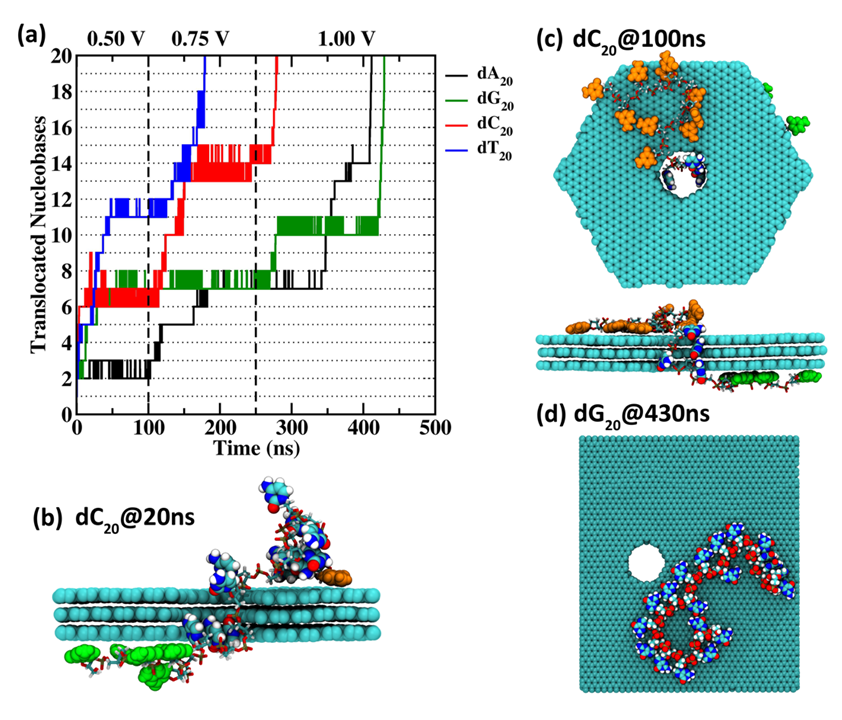
\includegraphics[width=\textwidth]{Chapter4/Figures/Figure3.png}
    \caption[DNA translocation through nanopores in a three-layer graphene membrane in additive FF]{DNA translocation through nanopores in a three-layer graphene membrane. (a) Number of translocated nucleobases as a function of simulation time obtained from additive (non-polarizable) simulations. Vertical dotted lines indicate change in the applied bias potential. (b) Representative snapshot of dC\textsubscript{20} recorded at 20 ns indicating the adhering of the 3’ end of the ssDNA onto the graphene surface. (c) Representative snapshot of dC\textsubscript{20} recorded at 100 ns indicating the adhering of the complete ssDNA onto the graphene surface. All nucleobases adhering to the top-graphene sheet are presented in orange, while those adhering to the bottom-graphene sheet are presented in green. (d) Representative snapshot of translocated dG\textsubscript{20} ss DNA.}
\end{figure}

To complete the translocation of the strands we increase the bias to 1.0 V. The increased bias resulted in a rapid step wise translocation of pyrimidine dC\textsubscript{20} within 280 ns. For the purine strands the higher bias restarts the translocation with stepwise nucleobase exits being observed between 340 ns and 410 ns for dA\textsubscript{20}, which is followed by a rapid exit from the nanopore with the last 6 nucleobases exiting within 5 ns. For dG\textsubscript{20} the increased bias relieves the pore clogging and translocation events are observed with nucleobases 8, 9, 10 translocating the nanopore. This is followed by a brief clogging period wherein nucleobases 10 and 11 remain trapped in the nanopore. However, once nucleobase 11 leaves the pore the remaining 9 nucleobases translocate within 5 ns, due to the significantly large bias. In Figure 6.3(d) we present a representative snapshot to illustrate the complete translocation of dG\textsubscript{20}. Following the translocation, the strand undergoes 2D diffusion on the graphene surface. 

\subsection{Drude Polarizable Simulations}
\begin{figure}
    \centering
    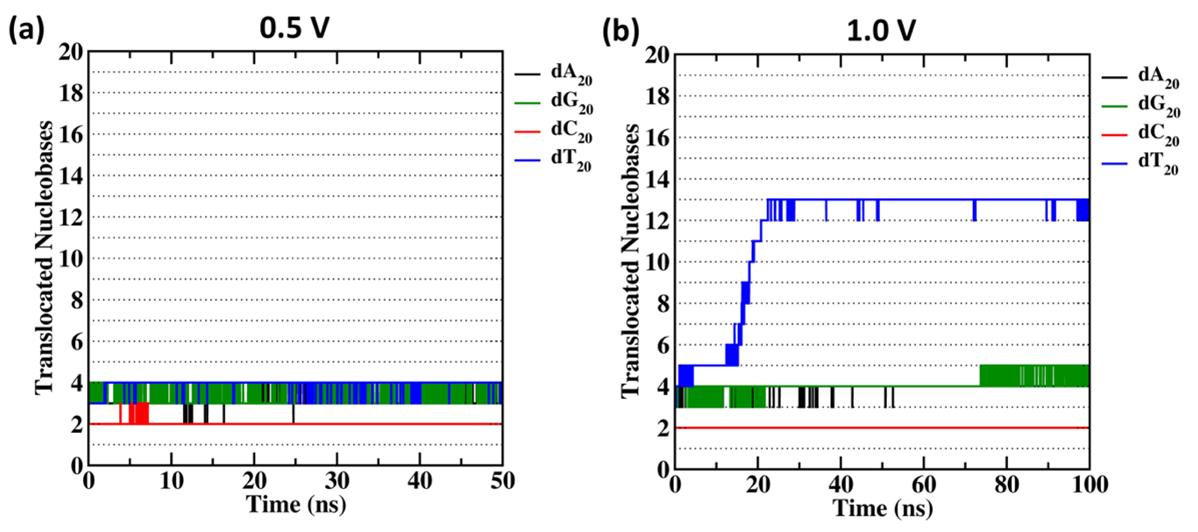
\includegraphics[width=\textwidth]{Chapter4/Figures/Figure12.png}
    \caption[Number of translocated nucleobases as a function of simulation time obtained from (a) 0.5 V and (b) 1.0 V Drude polarizable simulations.]{Number of translocated nucleobases as a function of simulation time obtained from (a) 0.5 V and (b) 1.0 V Drude polarizable simulations.}
\end{figure}

For the Drude simulations we did not observe any translocations for a bias voltage of 0.5 V. Translocations were observed only for dT\textsubscript{20} when the bias voltage was increased to 1.0 V. In Figure 6.4 we present the time series corresponding to simulations performed at 0.5 V and 1.0 V to illustrate our observations. Thus, in order to study the translocations of ssDNA we used higher bias voltages of 1.0 V (for 20 ns) followed by 1.5 V (for 80 ns) and 1.75 V till complete translocation or till the simulations reached 200 ns. In Figure 6.5(a) we present the timeseries of the translocation events observed in the Drude simulations. In the first 20 ns under the application of a bias voltage of 1.0 V we observe sequential translocations only for dT\textsubscript{20}, wherein 11 nucleobases translocate within the time window. Upon increasing the bias voltage to 1.5 V all the systems begin to translocate. The complete dT\textsubscript{20} strand crosses the nanopore within 27 ns. For dA\textsubscript{20} 9 nucleobases move through the nanopore within 37 ns following which we observe pore clogging till 100 ns. For dG\textsubscript{20} the pore remains clogged till 72 ns after which only one more nucleobase crosses the nanopore till 100 ns. The most sluggish translocation was observed for dC\textsubscript{20}, wherein the pore remined clogged till 80 ns and only 4 translocation events are recorded after that till 100ns. Upon further increase in the bias voltage to 1.75 V, we observe spontaneous translocation events. Complete translocation of dG\textsubscript{20} and dA\textsubscript{20} was observed within 125 ns and 161 ns respectively. For dG\textsubscript{20} rapid translocation was observed within $\approx$10 ns, with 15 nucleobases traversing the nanopore. While, for dA\textsubscript{20} the complete translocation was recorded over $\approx$61 ns, with 10 nucleobases traversing the nanopore. Interestingly, even under the application of the large external bias complete translocation was not observed for dC\textsubscript{20}. Only 12 cytosine nucleobases were found to translocate via the nanopore. We analyze the simulations trajectories to identify the molecular interactions governing the translocation dynamics. 

We observe that contrary to the additive (non-polarizable) simulations, the 3’ end of the ssDNA does not spontaneously tether to the graphene surface in Drude simulations. In Figure D.2 of the Appendix D we present the z-coordinate projection of the center of mass of the 3’-end nucleobases (18, 19 and 20) with respect to the top layer graphene sheet from the translocation 1.0 V – 1.5 V – 1.75 V simulations. In all the simulations we observe a significant slowdown in the tethering dynamics. We note that this is due to the formation of intra-strand H-bonds between the nucleobases in Drude simulations, due to the improved description of the H-bond dynamics in the polarizable force field.\supercite{lemkul_induced_2014} In Figure 6.5(b) and Table 6.1 we present the statistics of the average number of nucleobase-nucleobase H-bonds observed in the ssDNA from the both ssDNA-graphene and freestanding ssDNA simulations. In the presence of the graphene nanopore we observe a significant increase in the number of nucleobase-nucleobase H-bonds for dG\textsubscript{20}, dC\textsubscript{20} and dT\textsubscript{20}, with the effect being most prominent for dC\textsubscript{20}. In the presence of the graphene nanopore the number of nucleobase-nucleobase H-bonds in dC\textsubscript{20} is found to be 8.12 $\pm$ 1.90, while the same for free standing dC\textsubscript{20} is found to be 2.29 $\pm$ 1.18. We note that inter base H-bonds especially amongst cytosine bases, has been observed experimentally. It has been observed that cytosine nucleobases spontaneously self-assemble on solid state supports like Au(111)\supercite{otero_elementary_2008,wandlowski_structure_1996} and highly oriented pyrolytic graphene (HOPG).\supercite{xu_coadsorption_2006} Cytosine-Cytosine base pairing has also been observed for cytosine monophosphates,\supercite{li_full_2023} highlighting the propensity of cytosine-cytosine homo base pairing. Such self-assemblies of cytosine nucleobases were captured using polarizable simulations that could not be accessed via additive (non-polarizable) simulations.\supercite{h_capturing_2022} 
\begin{figure}
    \centering
    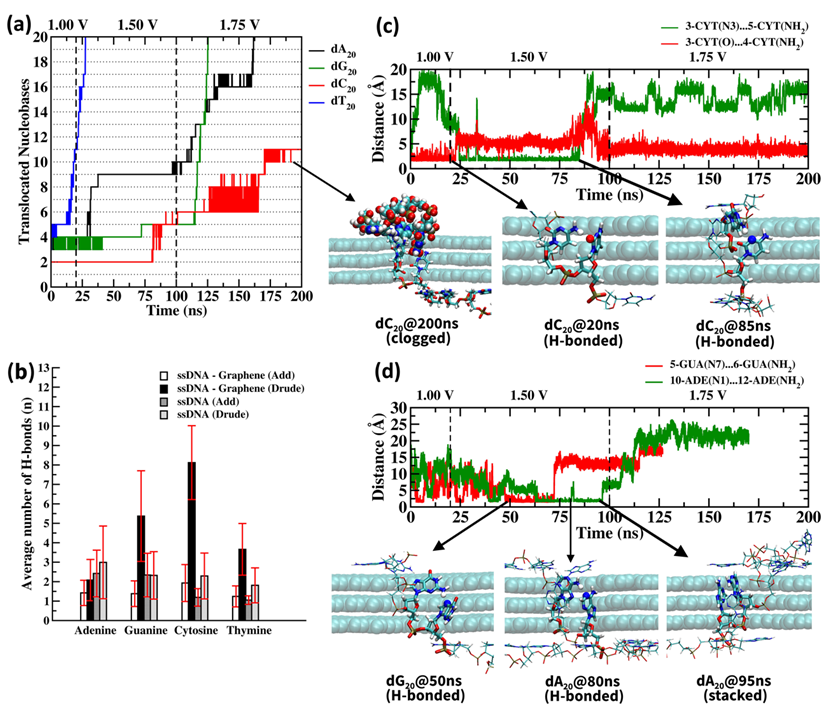
\includegraphics[width=\textwidth]{Chapter4/Figures/Figure4.png}
    \caption[DNA translocation through nanopores in a three-layer graphene membrane in Drude polarizable FF]{(a) Number of translocated nucleobases as a function of simulation time obtained from Drude simulations. Vertical dotted lines indicate change in the applied bias potential. (b) Average number of nucleobase-nucleobase H-bonds observed in ssDNA from ssDNA-graphene and freestanding-ssDNA additive (non-polarizable) and Drude polarizabe simulations. (c) Time series on inter-base H-bond responsible for the observed pore clogging in dC\textsubscript{20}. Representative snapshots illustrating the H-bond interactions are presented. Representative snapshot corresponding to the clogged state at 200 ns for dC\textsubscript{20} is also presented. (d) Time series of inter-base H-bond responsible for the observed pore clogging in dG\textsubscript{20} and dA\textsubscript{20}. Representative snapshots illustrating the H-bond interactions are presented for both dG\textsubscript{20} and dA\textsubscript{20}. Representative snapshot illustrating $\pi$-$\pi$ stacking in dA\textsubscript{20} is also presented. Time series are presented till the completion of translocation or till 200 ns for incomplete translocation.}
\end{figure}

\begin{table}[]
    \centering
    \caption[Average number of nucleobase-nucleobase H-bonds observed in the additive (non-polarizable) and Drude polarizable simulations.]{Average number of nucleobase-nucleobase H-bonds (n) observed in the additive (non-polarizable) and Drude polarizable simulations.}
    \label{tab:my-table}
    \resizebox{\textwidth}{!}{%
    \begin{tabular}{@{}ccllll@{}}
    \toprule
    \multicolumn{2}{c}{}                                           & \multicolumn{1}{c}{Adenine} & \multicolumn{1}{c}{Guanine} & \multicolumn{1}{c}{Cytosine} & \multicolumn{1}{c}{Thymine} \\ \midrule
    \multirow{2}{*}{additive (non-polarizable)} & ssDNA - graphene & 1.42 ± 0.65                 & 1.38 ± 0.66                 & 1.93 ± 0.95                  & 1.24 ± 0.54                 \\
                                                & ssDNA            & 2.42 ± 1.20                 & 2.34 ± 1.12                 & 1.19 ± 0.45                  & 1.05 ± 0.22                 \\
    \multirow{2}{*}{Drude polarizable}          & ssDNA - graphene & 2.08 ± 1.06                 & 5.37 ± 2.23                 & 8.12 ± 1.90                  & 3.66 ± 1.33                 \\
                                                & ssDNA            & 2.99 ± 1.87                 & 2.32 ± 1.22                 & 2.29 ± 1.18                  & 1.81 ± 0.90                 \\ \bottomrule 
    \end{tabular}%
    }
\end{table}

The confined dynamics of the ssDNA introduced upon interacting with the graphene nanopore contributes to the stabilization of the transient H-bonds observed amongst cytosines in dC\textsubscript{20}. For dC\textsubscript{20} these H-bonds were found to be responsible for the observed pore blockage in the Drude simulations. In Figure 6.5(c) we present the time series of H-bonds formed by 3-CYT with 4-CYT (3-CYT(N3) -- 4-CYT(NH\textsubscript{2})) and 5-CYT (3-CYT(O) -- 5-CYT(NH\textsubscript{2})) respectively. These H-bonds involving the acceptor atoms of 3-CYT and the donor atoms of 4-CYT and 5-CYT lock the position of 3-CYT within the pore, thus leading to the observed pore blockage till 80ns. In addition to the nucleobase-nucleobase H-bonds we also observe significant $\pi$-$\pi$ stacking amongst the nucleobases. Such $\pi$-stacks and nucleobase H-bonds stabilize the knot-like structure observed in dC\textsubscript{20}, which restricts the complete translocation of the strand. In Figure 6.5(c) we present a representative image of the knot-like structure observed between the terminal residues 15-CYT to 20-CYT for dC\textsubscript{20}. An inter-nucleobase H-bond observed within the nanopore also affects the translocation dynamics in dG\textsubscript{20} and dA\textsubscript{20}. In Figure 6.5(d) we present the time series corresponding to the H-bonds observed in dG\textsubscript{20} and dA\textsubscript{20}. Formation of a nucleobase-nucleobase H-bond between consecutive guanine’s 5-GUA and 6-GUA (5-GUA(N7) -- 6-GUA(NH\textsubscript{2})) traps these nucleobases within the nanopore, leading to the pore blockage. For dA\textsubscript{20} the nucleobase-nucleobase H-bond is observed between 10-ADE and 12-ADE (10-ADE(N1) -- 12-ADE(NH\textsubscript{2})), which stops the strand translocation. Interestingly this H-bond is also stabilized by $\pi$-$\pi$ stacking interaction between 10-ADE and 11-ADE. In Figure 6.5(d) we also present representative snapshots illustrating the H-bonding and $\pi$-stacking interactions. 

\subsection[Drude Polarizable Simulations (Lower Bias)]{Drude Polarizable Simulations (Lower Bias)}
\begin{figure}
    \centering
    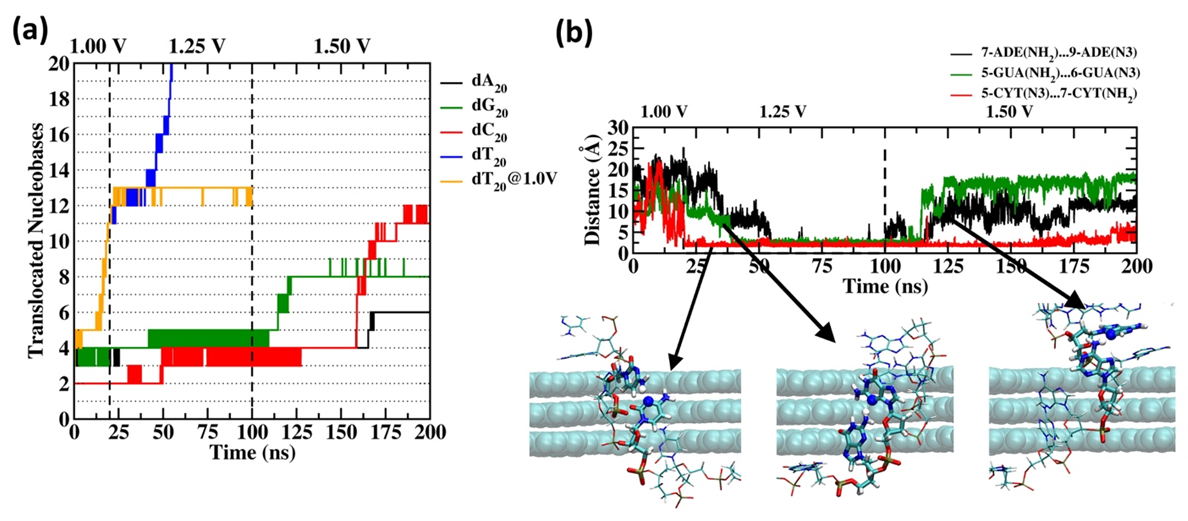
\includegraphics[width=\textwidth]{Chapter4/Figures/Figure5.png}
    \caption[DNA translocation through nanopores in a three-layer graphene membrane in Drude polarizable FF at lower voltages]{(a) Number of translocated nucleobases as a function of simulation time obtained from Drude simulations at lower bias voltages. Vertical dotted lines indicate change in the applied bias. (b) Time series of inter-base H-bond responsible for the observed pore clogging in dA\textsubscript{20}, dG\textsubscript{20}, and dC\textsubscript{20}. Representative snapshots illustrating the H-bond interactions are presented. All figures prepared using VMD.\supercite{humphrey_vmd_1996}}
\end{figure}

We note that the rapid nucleobase translocation observed for dT\textsubscript{20} and for dG\textsubscript{20} arises due to the large applied bias voltage of 1.5 V. Ideally, we require a slow and sequential translocation. In order to investigate the effect of the applied bias-voltage we ran additional simulations at lower bias conditions of 1.25 V for 80 ns following the initial 1.0 V runs of 20 ns. After the completion of 100 ns the bias voltage is increased to 1.5 V for additional 100 ns, resulting in a cumulative simulation time of 200 ns. In Figure 6.6(a) we present the timeseries of the translocation events observed in the Drude simulations. For dT\textsubscript{20} we observe a slowdown in the translocation dynamics under the application of a bias voltage of 1.25 V, with sequential translocations being observed from 20 ns till $\approx$ 60 ns, as compared to the rapid translocation observed in Figure 6.5(a). A bias voltage of 1.0 V was not enough to facilitate strand translocation for dT\textsubscript{20}. This indicates the requirement of ramping the bias voltage to facilitate strand translocation. For dA\textsubscript{20}, dG\textsubscript{20} and dC\textsubscript{20} we do not observe any significant translocation under the application of 1.25 V bias voltage. Strand translocation resumes under the application of 1.5 V bias voltage. However, within 200 ns we do not observe complete strand translocation. Similar, to the previous Drude simulations we observe that the formation of nucleobase-nucleobase H-bonds and $\pi$-$\pi$ stacking amongst the nucleobases is responsible for the pore clogging and sluggish translocation. In Figure 6.6(b) we present the timeseries corresponding to the H-bonds observed in dA\textsubscript{20}, dG\textsubscript{20} and dC\textsubscript{20} that are responsible for the pore clogging. For dC\textsubscript{20} and dG\textsubscript{20} the nucleobase-nucleobase H-bond responsible for the pore clogging is observed between the residues occupying the pore, while for dA\textsubscript{20} the H-bond is observed between residues outside the pore. We notice that the stability of H-bonds in dC\textsubscript{20} is significantly more when compared to dA\textsubscript{20} and dG\textsubscript{20}.

\subsection[Nanopore Occupancy]{Nanopore Occupancy}
\begin{figure}
    \centering
    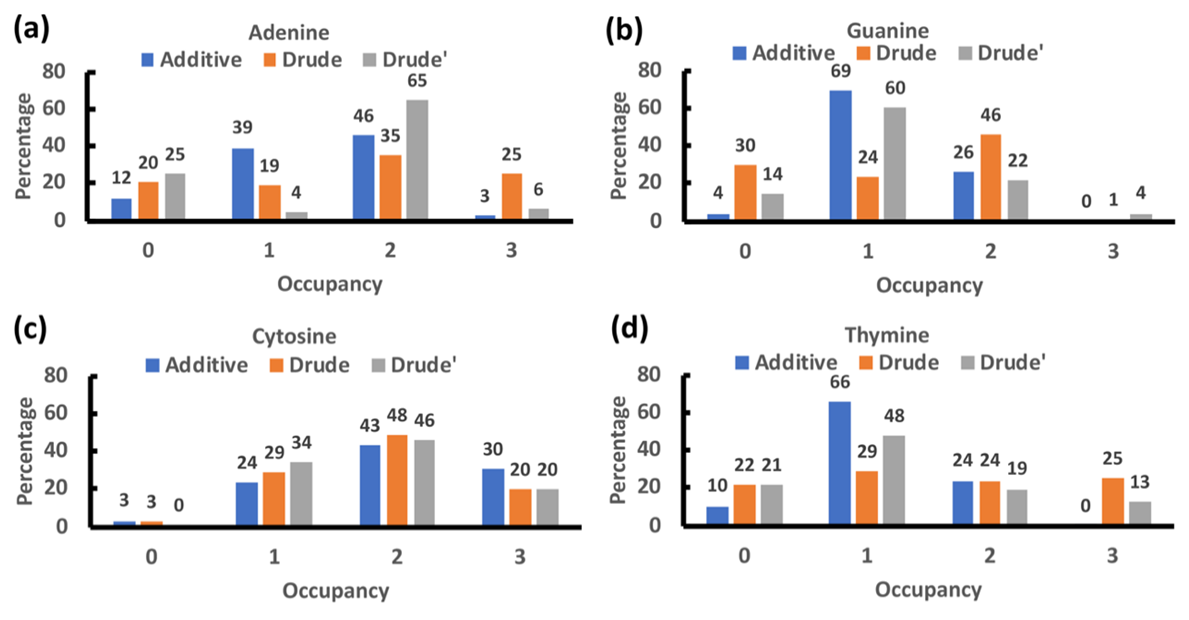
\includegraphics[width=\textwidth]{Chapter4/Figures/Figure6.png}
    \caption[Percentage of the number of nucleobases occupying the nanopore simultaneously evaluated from additive (non-polarizable) and Drude simulations for Adenine, Guanine, Cytosine and Thymine.]{Percentage of the number of nucleobases occupying the nanopore simultaneously evaluated from additive (non-polarizable) and Drude simulations for (a) Adenine, (b) Guanine, (c) Cytosine and (d) Thymine. Drude simulations performed using bias conditions 1.0V-1.50V-1.75V are labelled as Drude, while those performed using bias conditions 1.0V-1.25V-1.50V are labelled as Drude'.}
\end{figure}
One of the salient requirements of an ideal nanopore is a single nucleobase occupancy for making an accurate measurement. However, the analysis of the H-bonds and associated $\pi$-stacks reveals signatures of multiple nucleobase occupancies in the nanopore. To investigate this, we calculate the occupancy of the nanopore as a function of simulation time. In Figure 6.7 we present the statistics of the average nanopore occupancies observed in the additive (non-polarizable) and the two Drude nanopore simulations under different bias conditions. A nucleobase is recorded as occupying the nanopore if the z-coordinate of the center of mass of the nucleobase lies between the z-coordinate of the center of mass of the top and the bottom graphene sheets. The percentage occupancy is calculated with respect to the time taken for complete translocation of the ssDNA or the maximum simulation time in the case of incomplete translocation of the ssDNA. The additive (non-polarizable) simulations were found to exhibit a preference for single nucleobase occupancy of the nanopore, with a single nucleobase occupying the nanopore in dG\textsubscript{20} (69\%) and dT\textsubscript{20} (66\%). For dA\textsubscript{20} and dC\textsubscript{20} two nucleobases are observed to preferentially occupy the nanopore with the occupancy being 46\% and 43\% respectively. For the Drude simulations we observe a strong bias dependence on the occupancy of the nanopore. Under larger translocation bias (1.0V-1.50V-1.75V) we observe as strong preference of two nucleobases occupying the nanopore for all the systems, with the occupancy varying between 24\% to 48\%. We also observe a significant increase in three nucleobases occupying the nanopore for dA\textsubscript{20} (25\%), dC\textsubscript{20} (20\%) and dT\textsubscript{20} (25\%). We notice that this is due to the increased ionic current which induces rapid translocation. Upon lowering the translocation bias (1.0V-1.25V-1.50V) we observe an appreciable drop in the number of occurrences of three nucleobases occupying the nanopore simultaneously. While dA\textsubscript{20} (65\%) and dC\textsubscript{20} (46\%) favor two nucleobases occupying the nanopore, dG\textsubscript{20} (60\%) and dT\textsubscript{20} (48\%) favor one nucleobase occupying the nanopore. An appreciable shift in the percentage occupancy is also observed upon lowering the translocation bias, indicative of slower translocation dynamics. These observations highlight that lower bias favors single occupancy and slower translocation dynamics. However, lower bias also results in prolonged clogged states due to nucleobase-nucleobase H-bonds and $\pi$-$\pi$ interactions. 

\subsection[Orientation Analysis]{Orientation Analysis}
Theoretical calculations and experimental studies have shown that $\pi$-$\pi$ interactions influence the physisorption of the nucleobases onto the graphene surface.\supercite{varghese_binding_2009,umadevi_quantum_2011} The nucleobases are found to lie flat on top of the graphene surface. However, within the nanopore the nucleobases are surrounded by the hydrophobic carbon atoms of graphene. It is important to analyze how the nucleobases are oriented and located in the nanopore and if the presence of multiple nucleobases influences their orientation. First-principle calculations using a single nucleotide or nucleobase placed within single-layer graphene nanogap have alluded to the influence of the orientation of the nucleotide and the lateral position of the same on the tunneling current. However, these calculations are restricted to a single layer graphene sheet and typically within a passivated nanogap. Such calculations\supercite{prasongkit_transverse_2011} do not capture the $\pi$-$\pi$ interactions of the nucleobase/nucleotide with the curved nanopore cavity. 
\begin{figure}
    \centering
    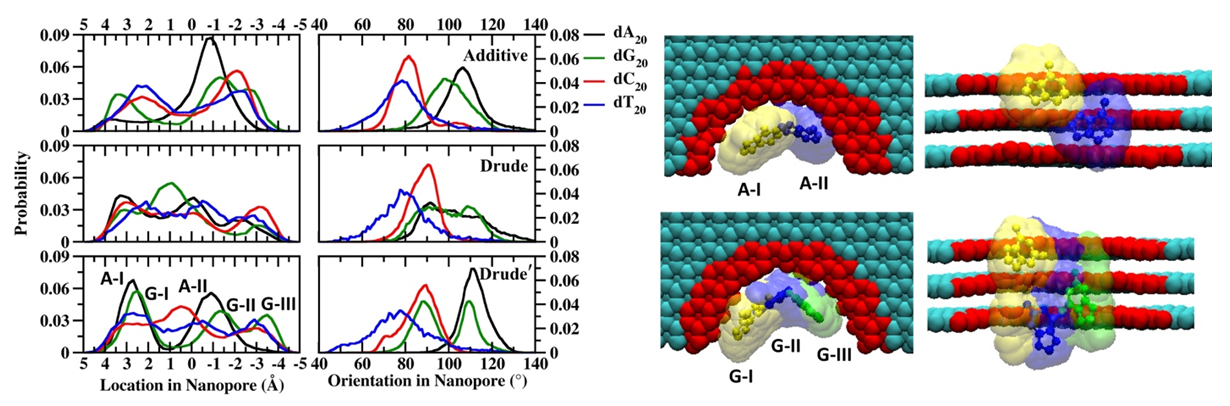
\includegraphics[width=\textwidth]{Chapter4/Figures/Figure7.png}
    \caption[Probability distribution of the location of the center of mass and the orientation of the nucleobase present within the nanopore evaluated from additive (non-polarizable) and Drude simulations]{Probability distribution of the location of the center of mass and the orientation of the nucleobase present within the nanopore evaluated from additive (non-polarizable) and Drude simulations. Drude simulations performed using bias conditions 1.0V-1.50V-1.75V are labelled as Drude, while those performed using bias conditions 1.0V-1.25V-1.50V are labelled as Drude'. Representative figures corresponding to the distance distributions observed for dA\textsubscript{20} (A-I and A-II) and dG\textsubscript{20} (G-I, G-II and G-III) are also presented. Pore edges are presented in red to highlight the curvature of the pore. The overall nucleobase probability distribution corresponding to each peak is accumulated and presented as surface representation. Representative nucleobases also presented in CPK representation to highlight the orientation of the nucleobase in the nanopore. All figures prepared using VMD.\supercite{humphrey_vmd_1996}}
\end{figure}

In Figure 6.8 we present the distributions corresponding to the two metrics which describe the nucleobase behavior in the nanopore, namely location of the nucleobase and the orientation of the nucleobase. The location of the nucleobase is described with respect to the center of mass of the nucleobase in the z-direction, while the orientation of the nucleobase is described as the angle between the surface normal of the nucleobase and the z-axis. In all the simulations we observe that the purine nucleobases, cytosine and thymine, do not exhibit a strong locational preference. Thymine nucleobases are observed to exhibit a very broad orientation preference, ranging from 40$\degree$ to 120$\degree$, with a peak that appears around $\approx$78$\degree$. Cytosine nucleobases on the other hand exhibit a strong orientation preference and are found to align nearly parallel to the surface of the nanopore cavity (or perpendicular to the surface normal of the graphene sheet) with the distribution being centered around $\approx$81$\degree$ for the additive (non-polarizable) dC\textsubscript{20} simulations and around $\approx$90$\degree$ for the two Drude dC\textsubscript{20} simulations. The pyrimidine nucleobases exhibit a locational preference based on the applied external bias. For the additive (non-polarizable) simulations, adenine shows a locational preference with a significant peak around -0.9 Å, which indicates localizing within the nanopore. For guanine we observe peaks around $\approx$ 3.5 Å, -1.0 Å and -3.0 Å, which is indicative of localizations near the pore entry, within the pore and pore exit. For both adenine and guanine, we observe a strong orientation preference with peaks centered around $\approx$106$\degree$ and $\approx$98$\degree$ respectively, indicative of aligning nearly parallel to the pore cavity. In the Drude simulations under the application of higher bias voltages, we do not observe any significant location or orientation preference, barring for cytosine nucleobases which still align themselves parallel to the nanopore cavity. This is indicative of the fast diffusion of the nucleobases through the cavity. Upon lowering the bias voltage, appreciable peaks are observed with both adenine (2.6 Å and -0.9 Å) and guanine (2.4 Å, -1.3 Å and -3.5 Å) favoring to reside in the cavity. Both adenine (110$\degree$) and guanine (88$\degree$ and 108$\degree$) favor aligning themselves parallel to the surface of the pore cavity. We notice that nucleobases tend to stick to the walls of the nanopore cavity while translocating through the nanopore. In Figure 6.9 we present the distribution of the center-of-mass of the nucleobase in the xy-plane, when residing within the nanopore. For dA\textsubscript{20}, dG\textsubscript{20} and dC\textsubscript{20} we observe distributions only closer to the walls of the nanopore. For dT\textsubscript{20} we observe distributions away from the nanopore walls, indicative of unrestricted movement of the thymine nucleobase through the nanopore. Similar unrestricted distributions are also observed under the application of elevated bias conditions (1.0V-1.50V-1.75V) in the Drude simulations. Upon lowering the bias (1.0V-1.25V-1.50V) we observe that the nucleobases (adenine, guanine and cytosine) adhere to the nanopore surface via $\pi$-$\pi$ interactions. We notice that the $\pi$-$\pi$ interactions play a significant role in governing the translocation dynamics. To quantify this interaction, we calculate the binding free energies of nucleosides and nucleotides interacting with the graphene surface. 
\begin{figure}
    \centering
    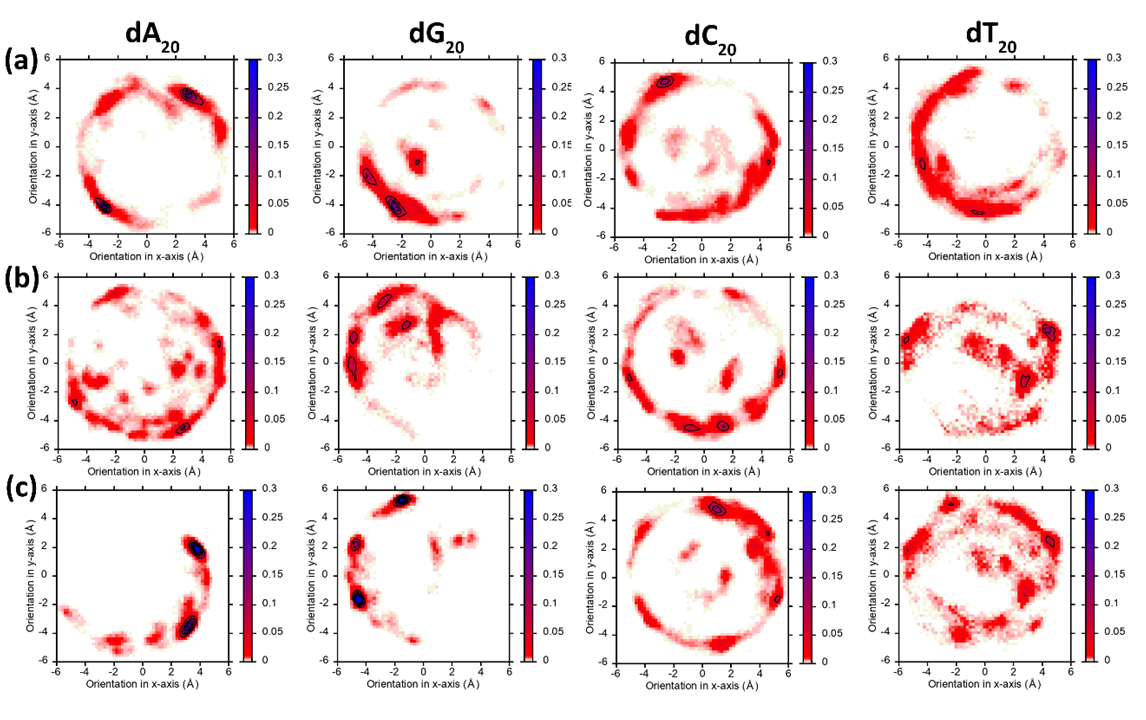
\includegraphics[width=\textwidth]{Chapter4/Figures/Figure8.png}
    \caption[2D distribution of the center-of-mass of the nucleobase in the xy-plane, when residing within the nanopore from additive, Drude and Drude' simulations]{2D distribution of the center-of-mass of the nucleobase in the xy-plane, when residing within the nanopore. (a) additive FF simulations, (b) 1.0 V - 1.50 V – 1.75 V Drude polarizable FF simulations, and (c) 1.0 V - 1.25 V – 1.50 V Drude polarizable FF simulations.}
\end{figure}

We now analyze the influence of staring conformation on the translocation dynamics of ssDNA through a pristine graphene nanopore using Drude Polarizable FF simulations.

\subsection[Influenece of Starting Conformation]{Influenece of Starting Conformation}
To investigate the effect of starting conformations on the translocation dynamics of ssDNA through graphene nanopores, we performed additional simulations for dA\textsubscript{20}, dG\textsubscript{20}, dC\textsubscript{20} and dT\textsubscript{20} using Drude polarizable FF, starting from a different conformation than the original simulations. The ssDNA strands were regenerated using the topology information present in the CHARMM nucleic acid force field.\supercite{baker_development_2011,savelyev_all-atom_2014} The procedure as described in the methods section was used to generate the graphene sheet. The initial conformation of the ssDNA was now created such that 5 nucleotides at the 5’-end of the ssDNA were threaded through the nanopore as opposed to 3 nucleotides as in the simulations presented in the Drude simulations. A different random seed was chosen to initialize the velocities in the NAMD simulations, thereby creating a different trajectory. The initial system geometry constructed is illustrated in Figure 6.10. The remaining simulations parameters are similar to the those reported in the methods sections.
\begin{figure}
    \centering
    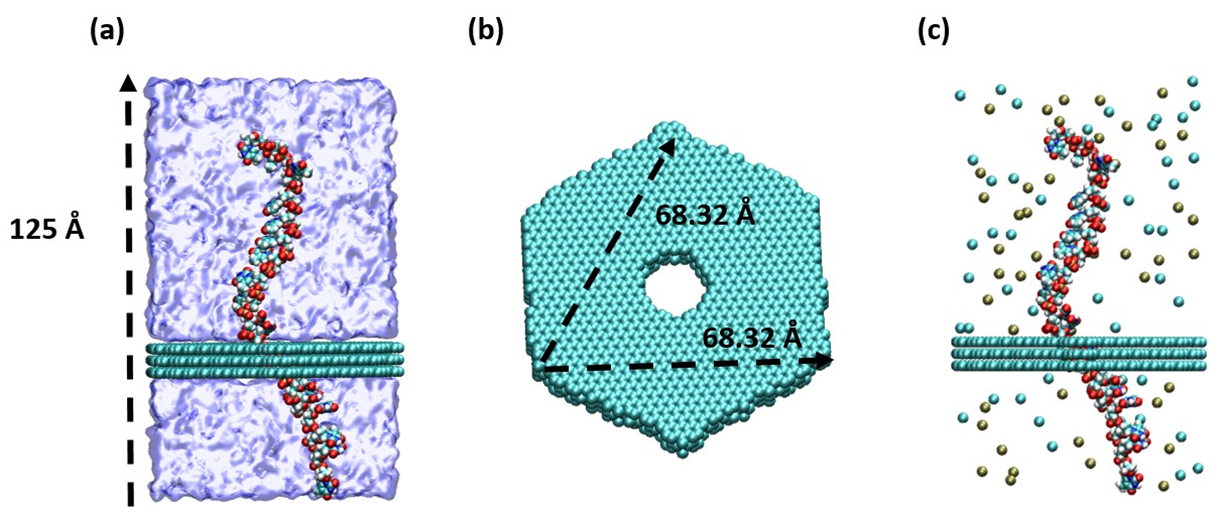
\includegraphics[width=\textwidth]{Chapter4/Figures/Figure9.png}
    \caption[Representative structures depicting the system setup for ssDNA – multilayer graphene.]{Representative structures depicting the system setup for ssDNA – multilayer graphene. Five nucleobases have been threaded through the nanopore, instead of three in the original simulations. (a) Side View and (b) Oblique view of the multilayer graphene to indicate periodic boundary conditions employed. (c) Complete ssDNA – multilayer graphene (water molecules are removed for clarity). All figures are prepared using VMD.\supercite{humphrey_vmd_1996}}
\end{figure}

We present the number of translocated nucleobases as a function of time in Figure 6.11. As reported in the Drude simulations, we apply a bias voltage of 1.0V for the first 20 ns, followed by increasing the applied external bias to 1.50 V for the next 80 ns. After the completion of cumulative 100 ns the applied external bias was increased to 1.75 V in an attempt to drive the complete translocation. 
\begin{figure}
    \centering
    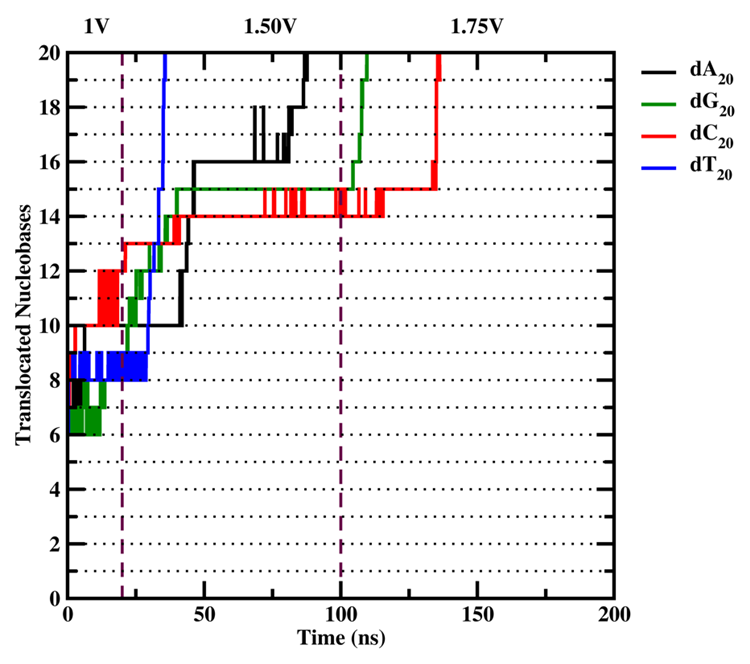
\includegraphics[width=0.75\textwidth]{Chapter4/Figures/Figure10.png}
    \caption[DNA translocation through nanopores in a three-layer graphene membrane in Drude polarizable FF starting from a different conformation]{Number of translocated nucleobases as a function of simulation time obtained from Drude simulations. Vertical dotted lines indicate change in the applied bias potential.}
\end{figure}

The translocation dynamics of dT\textsubscript{20} shows very similar characteristics to the original Drude simulations. We note that the 8\textsuperscript{th} and 9\textsuperscript{th} nucleotides undergo a ratcheting motion within the nanopore during the first 20 ns of the simulation. This state rapidly gives way to rapid translocation of the remaining 11 nucleotides once the applied external bias is increased to 1.50 V. We observe that the remaining 11 nucleotides undergo translocation in rapid succession within the next $\approx$ 5 ns, once the 8\textsuperscript{th} and 9\textsuperscript{th} nucleotides exited the nanopore at around 25 ns. We note that for dA\textsubscript{20}, rapid translocation of four nucleotides is completed within the first $\approx$10 ns of the simulation time, and the translocations then approach a plateau, with no further translocations observed till the applied external bias was increased to 1.50V at the end of the first 20 ns. As we increased the applied external bias to 1.50V, we observed the appearance of translocations again in dA\textsubscript{20}, with $\approx$6 nucleobases rapidly exiting the nanopore once the translocation got initiated at $\approx$45 ns. During this translocation window, we note the instances of two nucleobases simultaneously exiting the nanopore (11 and 12) and (14 and 16). This short translocation was followed by the appearance of another clogged state, spanning the next 15 ns of the simulation time. This clogged state was relieved towards the end of 75 ns, where the remaining nucleobases exit the nanopore in a step-wise fashion. For dG\textsubscript{20}, we observe that the nucleobases 7 and 8 undergo a ratcheting motion during the first 15 ns of the simulation time, culminating in them exiting the nanopore in quick succession towards the end of the first 15 ns. Once the applied external bias was increased to 1.50V, we observe a smooth translocation of nucleobases in dG\textsubscript{20}, with nearly 7 nucleobases exiting the nanopore in the next 20 ns of the simulation. This window of translocation was followed by the appearance of a clogged state, spanning the next 60 ns of the simulation time. After the first 100 ns of the simulation, an increase in the applied external bias to 1.75V resulted in the remaining nucleobases exiting the nanopore in rapid succession. For dC\textsubscript{20}, we note that three nucleobases (6, 7 and 8) undergo rapid translocations during the first few nanoseconds, followed by the nucleobases 11 and 12 undergoing a ratcheting motion within the nanopore. This state is relieved once both the nucleobases simultaneously exit the nanopore at 20 ns mark, when the applied external bias was increased to 1.50V. We observed the translocation of $\approx$ 2 more nucleobases within the next 80 ns of the simulation time. Towards the end of the first 100 ns of the simulation, an increase in the applied external bias to 1.75V drives the translocation process to completion. 

On comparing the translocation dynamic with the previous set of runs, we observe the same trend with dT\textsubscript{20} exhibiting the fastest translocation through the nanopore and dC\textsubscript{20} exhibiting the slowest translocation. dA\textsubscript{20} and dG\textsubscript{20} present translocation dynamics which are intermediate between the dT\textsubscript{20} and dC\textsubscript{20}. One of the main difference between the nanopore dynamics was the translocation of $\approx$ 3-4 nucleotides within the first 20 ns of the simulation. In contrast, we did not observe significant translocations during the first 20 ns in the original simulations as seen in Figure 6.5(a). This is due to the increased number of nucleobases on the trans side (bottom) of the nanopore in these simulations when compared to the previous simulations which pull a part of the strand towards the trans side before the remainder of the strand falls adheres to the graphene sheet on the cis side (top). Once the strand adheres to both the cis and the trans side of the nanopore the translocation dynamics is stalled as observed in the previous simulations. The translocation is restarted only on the application of an external bias. 

\begin{figure}
    \centering
    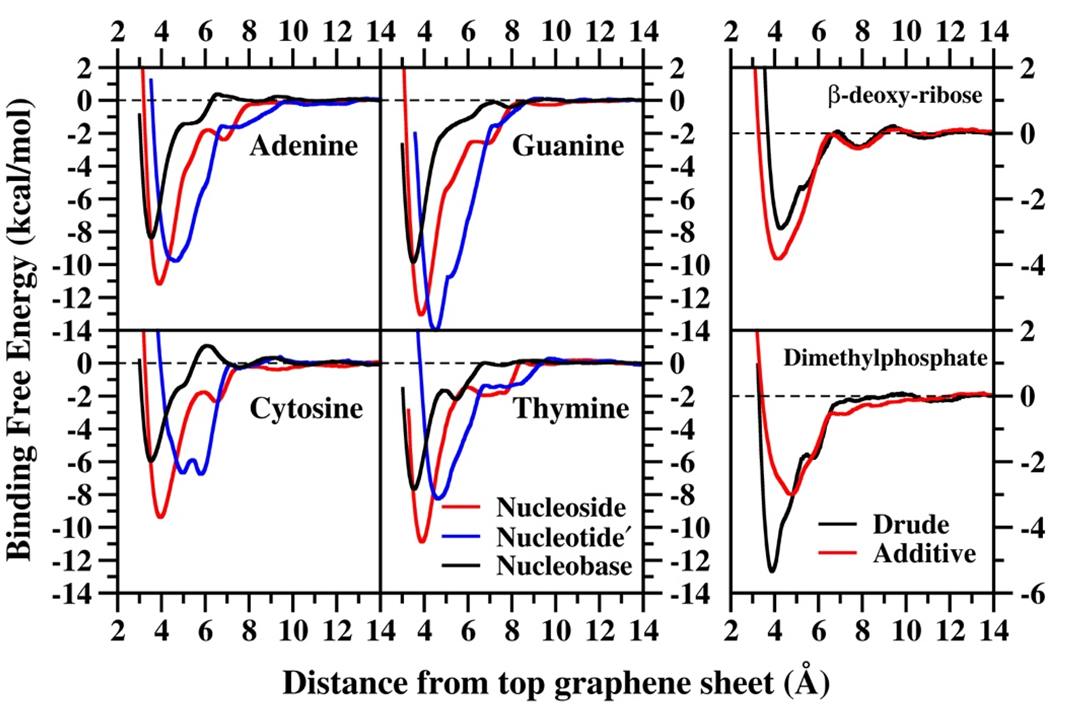
\includegraphics[width=\textwidth]{Chapter4/Figures/Figure11.png}
    \caption[Potential of mean force (PMF) for nucleobase, nucleoside, nucleotide´, $\beta$-deoxy ribose and dimethyl phosphate interacting with the graphene surface obtained from Drude simulations.]{Potential of mean force (PMF) for nucleobase, nucleoside and nucleotide´ interacting with the graphene surface obtained from Drude simulations. PMF for $\beta$-deoxy ribose and dimethyl phosphate interacting with the graphene surface obtained from additive (non-polarizable) and Drude simulations are also shown. All distances are presented in Å and binding free energies in kcal/mol. PMF for nucleobases are reproduced from our earlier study.\supercite{h_polarization_2021} Nucleotide´ corresponds to a modified nucleotide with phosphates at the 3’ and 5’ ends passivated by methyl groups to mimic the sugar-phosphate backbone.}
\end{figure}
\begin{landscape}
    \normalsize
    \begin{table}
        \centering
        \caption[Binding free energies obtained from Drude ABF simulations and experimental studies for nucleobases, nucleosides and nucleotides]{Binding free energies obtained from Drude ABF simulations. Binding energies are calculated as the difference between the energies of the equilibrium structure and the well-separated structure. Binding energies for nucleobases and nucleosides estimated from ITC measurements by Rao et. al.\supercite{varghese_binding_2009} and Chen et. al.\supercite{ranganathan_complex_2016} respectively. Binding energies for nucleotides estimated from SMFS experiments by Vezenov et. al\supercite{manohar_peeling_2008,iliafar_quantifying_2012} and Walsh et. al\supercite{hughes_adsorption_2017}}
        \label{tab:my-table}
        \begin{tabular}{@{}cccccccc@{}}
        \toprule
        \multicolumn{1}{c}{} & \multicolumn{3}{c}{Drude FF (kcal/mol)} & \multicolumn{4}{c}{Expt. (kcal/mol)}                   \\ \midrule
        System                 & Nucleobase\supercite{h_polarization_2021}  & Nucleoside  & Nucleotide'  & Nucleobase\supercite{varghese_binding_2009} & Nucleoside\supercite{ranganathan_complex_2016} & Nucleotide\supercite{manohar_peeling_2008,iliafar_quantifying_2012} & Nucleotide\supercite{hughes_adsorption_2017}   \\ \midrule
        Adenine                & -8.35       & -11.18      & -9.79        & -11.85     & -6.0       & -5.87      & -9.0         \\
        Guanine                & -8.93       & -13.06      & -14.02       & -13.45     & -6.2       & -4.92      & -12.67       \\
        Cytosine               & -5.96       & -9.39       & -6.75        & -9.38      & -5.8       & -4.48      & -7.65        \\
        Thymine                & -7.66       & -10.88      & -8.26        & -4.72      & -5.1       & -6.70      & -7.89                         
        \end{tabular}
    \end{table}  
\end{landscape}
\subsection[Binding Free Energies]{Binding Free Energies}
In Figure 6.12 we present potential of mean force (PMF) scans obtained from the Drude polarizable ABF simulations for nucleobase, nucleoside and nucleotide´ interacting with the graphene surface. The nucleobase PMF scans have been reproduced from our previous study wherein we investigated the binding free energies for purine and pyrimidine nucleobases interacting with the graphene surface.\supercite{h_polarization_2021} In Figure 6.6 we also present the PMF scans obtained for $\beta$-deoxy-ribose and dimethyl phosphate interacting with the graphene sheet from additive (non-polarizable) and Drude ABF simulations. Similar to the previous study, the scan coordinate was chosen to be the z-coordinate projection of the center-of-mass of the nucleobase, nucleoside, nucleotide´, sugar or dimethyl phosphate with respect to the top-most graphene sheet. In Table 6.2 we present the binding free energies estimated from the PMF scans. We note that the binding free energies follows an interaction pattern of G > A > T > C, with the purine’s binding strongly to the graphene sheet when compared to the pyrimidine’s irrespective of whether we study a nucleobase, nucleoside or nucleotide´. For all systems other than guanine we observe that the binding energies follow the trend nucleoside > nucleotide´ > nucleobase. For guanine we observe that the nucleotide´ (-14.02 kcal/mol) binding is favored over the nucleoside (-13.06 kcal/mol). The results indicate that the presence of sugar and charged phosphate backbone aids in the binding of the nucleoside and nucleotide to the graphene sheet. From Figure 6.12 we observe that the presence of the bulky sugar in the nucleoside and the sugar-phosphate groups in the nucleotide´ shifts the location of the minima to higher values. The minima for the nucleobases are observed around 3.5 Å, while the same for the nucleosides is observed around 3.9 Å. The shift is due to the presence of the sugar group. The presence of the sugar unit however does not severely affect the $\pi$-$\pi$ interactions between the nucleobase and the graphene sheet. For the nucleotide´ the minima appear around 4.6 Å for Adenine, Guanine and Thymine, while it appears around 5.8 Å for Cytosine. We note that the presence of the ribose-phosphate backbone influences the $\pi$-$\pi$ interaction between the nucleobase and the graphene sheet, with the presence of the phosphate group influencing the desorption of the nucleotide when compared to the nucleoside. These observations are in line with experimental estimates of nucleoside and nucleotide binding energies. Using iso-thermal calorimetry (ITC) experiments Chen et. al. reported binding free energy values of adenosine, guanosine, cytidine and thymidine interacting with nanoscale Graphene oxide (nGO) to be -6.0 kcal/mol, -6.2 kcal/mol, -5.8 kcal/mol and -5.1 kcal/mol.\supercite{ranganathan_complex_2016} These values qualitatively agree with the trend observed by us wherein G > A > T > C. In addition to studying the nucleosides Chen at. al. also investigated the binding of short single stranded DNA oligonucleotides with nGO.\supercite{ranganathan_complex_2016} The order of the association constants for the short oligonucleotides was found to be CCCCC $\approx$ AAAAA > AGCTA > TTTTT. Data could not be obtained for GGGGG due to strong non-covalent interactions between guanine bases. It must be noted that the binding free energies were obtained for nucleosides interacting with nanoscale flakes of graphene oxide. These substrates can be significantly different from pristine graphene or HOPG surfaces. This can explain the observed differences in the values obtained from PMF simulations and the ITC measurements. We note that the adsorption energies for nucleobase-graphene interactions obtained from Drude simulations agree with ITC derived energies for nucleobases interacting with graphene surfaces as reported by Rao et. al.\supercite{varghese_binding_2009}, highlighting differences between nGO and HOPG surfaces. 

However, the experimental observations agree with the trends obtained by Drude simulations. Guanine favors significant $\pi$-$\pi$ interactions as evidenced by the significant time taken for the 3’ end to adhere to the graphene surface in the Drude simulations [Figure D.2]. Thymine was observed to translocate fastest through the nanopore, the observation being consistent with the smaller association constant for TTTTT. This differentiation between nucleotides is not captured in the additive (non-polarizable) simulations. Chen et. al. also studied the binding of dA\textsubscript{15} with nGO.\supercite{ranganathan_complex_2016} They observed an increase in the binding affinity of dA\textsubscript{15} when compared to dA\textsubscript{5}, however they observed that the increase did not correspond to all the nucleobases interacting with the graphene surface. They concluded that in addition to interacting with the graphene surface the nucleobases were also involved in intra-strand stacking interactions. We notice that such a behavior is only observed in the Drude simulations, while in additive (non-polarizable) simulations all the nucleobases are observed to adhere to the graphene surface.

Binding free energy per nucleotides can also be estimated using single-molecule force spectroscopy (SMFS). Using SMFS, Vezenov et. al estimated the binding free energies for adenine (dA\textsubscript{50}), guanine (dG\textsubscript{100}), cytosine (dC\textsubscript{50}) and thymine (dT\textsubscript{50}) interacting with graphene surface to be -5.87 kcal/mol, -4.92 kcal/mol, -4.48 kcal/mol and -6.70 kcal/mol.\supercite{manohar_peeling_2008,iliafar_quantifying_2012} These results indicated a stronger binding for the thymine strand compared to guanine and cytosine. In a more recent study, Walsh et. al. estimated the binding free energies for adenine (dA\textsubscript{30}), guanine (dG\textsubscript{30}), cytosine (dC\textsubscript{30}) and thymine (dT\textsubscript{30}) interacting with graphene using SMFS to be -9.0 kcal/mol, -12.67 kcal/mol, -7.65 kcal/mol and -7.89 kcal/mol.\supercite{hughes_adsorption_2017} These results are more in line with the trends observed in the ABF simulations with G > A > T $\approx$ C. Vezenov et. al noted that the estimated binding free energies might be influenced by the formation of higher order secondary structures like knots in the long oligomers (50 or 100) used in the SMFS experiments.\supercite{manohar_peeling_2008,iliafar_quantifying_2012} Additionally, it must be noted that SMFS experiments use a non-equilibrium pulling process to describe an equilibrium binding event. This inherently includes assumptions, which can affect the absolute values of the binding free energies. These experiments present a trend which agrees with the observations from simulations, especially for the shorter dA\textsubscript{30}, dG\textsubscript{30}, dC\textsubscript{30} and d\textsubscript{30} oligo-nucleotides. 

Before summarizing our observations, we comment on the binding free energies for the phosphate group. Binding free energies for dimethyl phosphate from Drude and additive (non-polarizable) FF simulations are -5.37 kcal/mol and -3.04 kcal/mol. This represents a stabilization of -2.33 kcal/mol in the Drude simulations when compared to the additive (non-polarizable) simulations. This shift in interaction energies is also accompanied by a shift in the location of the interaction minima, with Drude polarizable FF predicting a closer interaction with the graphene sheet at 3.88 Å, while additive (non-polarizable) FF predicts the interaction minima to be at distance of 4.80 Å from the graphene surface. This shift in the interaction energies, and the minima are due to the differences in the interactions that are being captured by additive (non-polarizable) and Drude polarizable FF simulations. In additive (non-polarizable) FF simulations, due to the graphene surface being approximated as a pure VdW surface, the minima accounts for the maximum VdW interaction between the graphene surface and the dimethyl phosphate molecule. However, in Drude polarizable FF simulations, the graphene surface is able to respond to the changes in the local environment, specifically the negative charge on the phosphate, leading to the accurate capture of both VdW and electrostatic interactions between the dimethyl phosphate molecule and the graphene surface. Drude polarizable simulations were able to capture similar interactions between the negatively charged Cl- ion and the graphene surface, which could not be captured by additive (non-polarizable) simulations.\supercite{h_capturing_2023} Using batch adsorption experiments Vasudevan et. al have shown that graphene has excellent phosphate adsorption properties.\supercite{vasudevan_adsorption_2012} They observed that the interaction of phosphate with the graphene surface was highly endothermic and a spontaneous process. The binding free energies obtained from our Drude FF simulations are in line with these observations.

\section[Conclusions]{Conclusions}
Based on the above discussions we present an overall insight into the translocation dynamics of ssDNA using pristine graphene nanopores. Four factors are found to govern the translocation dynamics; (i) $\pi$-$\pi$ interactions between the nucleobases and the graphene surface (ii) intra-strand dynamics: H-bonding and $\pi$-stacking, (iii) electrostatic interactions between the charged phosphate backbone and the graphene surface and (iv) applied external bias. In Figure 6.13 we present a schematic describing the progress of the translocation dynamics and how these interactions influence the same using representative snapshots from the various simulation trajectories. 
\begin{figure}[!h]
    \centering
    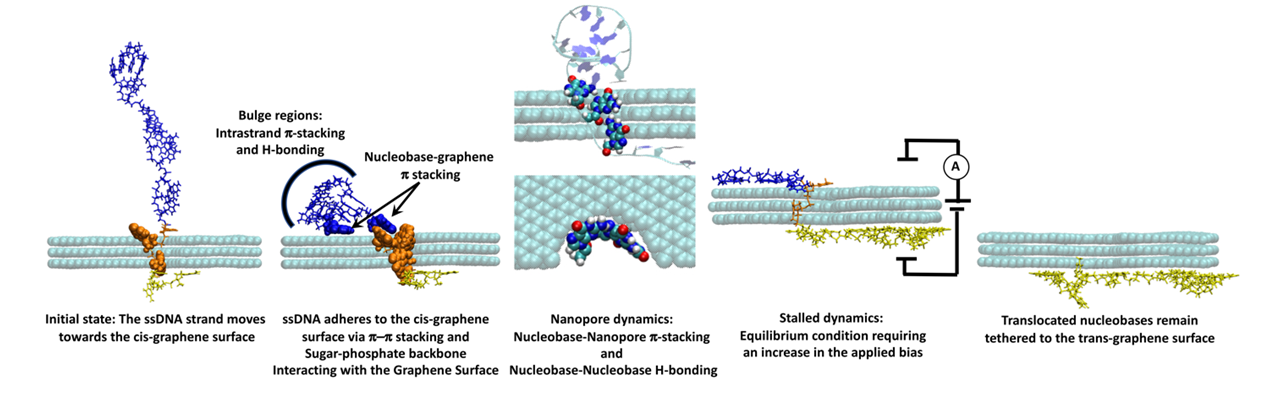
\includegraphics[width=\textwidth]{Chapter4/Figures/Figure_last.png}
    \caption[Schematic figure illustrating the progress of the translocation dynamics and how the various interactions influence the translocation dynamics]{Schematic figure illustrating the progress of the translocation dynamics and how the various interactions influence the same. Nucleobases on the cis side of the nanopore, within the nanopore and the trans-side of the nanopore are presented in blue, orange and yellow respectively. Nucleobases interacting with the graphene sheet via $\pi$-$\pi$ interactions are presented in VdW representation.}
\end{figure}

The $\pi$-$\pi$ interactions between the nucleobases and the graphene surface control the overall translocation dynamics. As a first step, these interactions are responsible for the ssDNA to adhere to the graphene surface. Depending on the size of the strand and the available surface area of graphene for binding, all the nucleobases can either adhere to the surface of graphene or bulge regions might appear wherein parts of the strand do not adhere to the graphene surface.\supercite{varghese_binding_2009, iliafar_quantifying_2012, manohar_peeling_2008, ranganathan_complex_2016} In addition to bulge regions longer ssDNAs are also prone to formation of transient and stable secondary structures which might impede the binding of the strand to the graphene surface. This is especially true for guanine rich sequences which can form quadruplex structures\supercite{spiegel_structure_2020} or cytosine rich sequences which might form intra-strand H-bonds\supercite{berger_inter-strand_1996}. It is observed that $\pi$-$\pi$ stacking interactions and nucleobase-graphene interactions are stronger for purines when compared to the pyrimidines. We note that the formation of secondary structures is strongly dependent on the DNA sequence. While our conclusions are based on the homo-polymer sequences the same results cannot be directly extrapolated to hetero-polymer sequences. Capturing these effects is crucial to describing the translocation dynamics. Additionally, we have observed that electrostatic interaction between ribose-phosphate backbone and the graphene sheet also slows down the translocation dynamics. An effect which is not captured in additive (non-polarizable) simulations. 

The dynamics in the nanopore are largely governed by $\pi$-$\pi$ interactions of the nucleobase to the hydrophobic curved surface of the nanopore. All nucleobases were found to adhere to the wall favoring a perpendicular orientation with respect to the surface normal of the graphene sheet. Thus, the nucleobases do not translocate through the middle of the nanopore as envisaged in earlier experimental studies. This also explains why no significant change were observed in the translocation dynamics upon increasing the pore-size\supercite{garaj_graphene_2010,merchant_dna_2010, schneider_dna_2010, schneider_tailoring_2013} in experimental studies. The localization in the hydrophobic cavity also favors secondary H-bond interactions which can arrest the translocation dynamics. Nucleobases trapped within the nanopore can be unbound upon increasing the external bias. 

Change in the external bias increases the ionic drift influencing the  translocation dynamics.  We observe that a large bias is detrimental towards nanopore sensing due to rapid translocation and multiple translocation events occurring simultaneously which affects their detection. For a slow stepwise translocation, it is preferred to apply very low external bias, just enough to create an ionic drift to facilitate the translocation. However, the translocated nucleobases remain tethered to the graphene surface. Due to this nature of translocation once half of the strand is translocated, we reach an equilibrium condition wherein close to similar number of nucleobases are adhered to both the top and bottom graphene sheets under low external bias. In such a scenario the translocation dynamics is paused and can be reinitiated only upon increasing the external bias or incorporating bias pulses. This problem gets compounded with increasing size of the ssDNA since multiple pauses in the translocation events are observed. Such pore clogging has been observed in experimental studies and relieving the clogged states is a significant challenge faced for using graphene as a nanopore.\supercite{garaj_graphene_2010,merchant_dna_2010, schneider_dna_2010, schneider_tailoring_2013}

Tuning the hydrophobicity of the graphene surface has been suggested as one of the ways to alleviate the issues associated with pore clogging. To investigate this, Dekker et. al. created a hydrophilic monolayer of aminopyrene interacting with a N-hydroxysuccinimide derivative of a 4-mer ethylene glycol.\supercite{schneider_tailoring_2013} In the resultant chemical moiety, it was envisaged that the pyrene sticks onto the graphene surface via $\pi$-$\pi$ interactions while the protruding ethylene glycol acts as the hydrophilic layer. No pore clogging events were observed in this non-covalently surface modified graphene nanopore, thus making this a viable strategy. The fact that various device architectures can be made from graphene and allied 2D materials remains the strongest claim for exploiting these systems for nanopore applications. Utilizing the presence of step defects in graphene and the associated mobility of DNA strands along the defect line Aksimentiev et. al. suggested using a spiral step pattern to guide a DNA strand towards the nanopore and away from it.\supercite{shankla_step-defect_2019} Dekker et. al. exploited the 2D nanoslit architecture in graphene and hexagonal boron nitride sheets to study the passage of DNA through the nanoslits akin to a nanopore.\supercite{yang_translocation_2021} The fact that multiple device architectures can be created using graphene highlights the need for an accurate description of the interactions between DNA and graphene. 

In summary, our study demonstrates the efficacy of Drude polarizable force field simulations in faithfully capturing the dynamic interactions between the single-stranded DNA (ssDNA) and both the graphene surface and nanopore environment. Our findings corroborate the experimental findings of Dekker et al., where analogous clogging behavior of ssDNA was observed and subsequently alleviated through the application of a high external bias.\supercite{schneider_tailoring_2013}  Notably, the Drude simulations are able to aptly replicate the formation of bulge regions in ssDNA, a phenomenon also observed in independent isothermal titration calorimetry (ITC) experiments\supercite{ranganathan_complex_2016} and single-molecule force spectroscopy (SMFS) measurements.\supercite{manohar_peeling_2008, iliafar_quantifying_2012,hughes_adsorption_2017} This observation is pivotal when extrapolating outcomes from shorter homopolymeric chains to longer sequences.

Importantly, our investigation reveals the pivotal role of intra-strand hydrogen bonding interactions in influencing nanopore translocation dynamics. Remarkably, these nuanced insights remained elusive in the  conventional additive (non-polarizable) simulations, which also underestimated the intricate dynamics of pore clogging. Thus, our study underscores the necessity of both disrupting ssDNA tethering to the solid-state substrate and perturbing intra-strand interactions for the effective design of solid-state nanopore devices. These findings collectively emphasize the significant merits of Drude polarizable simulations in unlocking molecular-level insights into nanopore behavior. We anticipate that our work will serve as a catalyst for the broader adoption of polarizable simulations in the exploration of interconnected interfacial phenomena. By unveiling the intricate interplay of forces and interactions, polarizable simulations stand poised to revolutionize our understanding of nanopore dynamics and their applications.